\begin{flushright}
    با انتزاع توانستیم از مدارات متشکل از ترانزیستور، گیت‌های منطقی را تعریف کنیم.
    حال می‌توانیم با استفاده از این گیت‌ها مدارات مجمتع مختلفی ایجاد کنیم.
    به طور مثال مدار شکل زیر متشکل شده از یک گیت xor و یک گیت or می‌باشد.

    \begin{figure}[h]
        \centering
        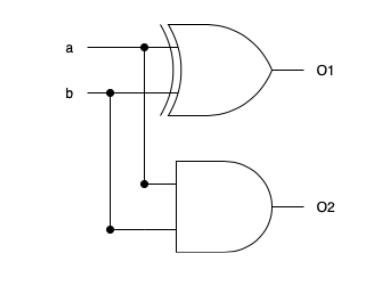
\includegraphics[width= 0.4\textwidth]{source/half-adder-imp}
        \caption{پیاده‌سازی مدار مجتمع نیمه‌جمع‌کننده}
        \label{fig:half-adder-imp}
    \end{figure}

    همانطور که از درس مدارمنطقی به یاد دارید، در نگاه \textbf{انتزاع} این مدار در عمل دو مقدار تک بیتی را جمع کرده و یک بیت حاصل جمع به همراه یک بیت نقلی را خروجی می‌دهد.
    به بیان دیگر شکل 3 یک \textbf{پیاده‌سازی} از نیمه‌جمع‌کننده می‌باشد.

    \begin{figure}[h]
        \centering
        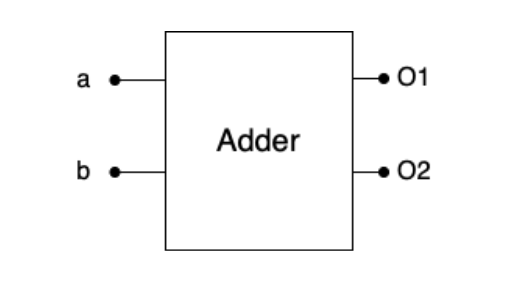
\includegraphics[width= 0.4\textwidth]{source/half-adder-abs}
        \caption{پیاده‌سازی مدار متشکل از دو گیت xor و or}
        \label{fig:half-adder-abs}
    \end{figure}

\end{flushright}